\section{Zbiór Wine}
\subsection{Algorytm Adaboost}

\begin{tabular}{llrrrrrrrr}
\hline
          & \{\} & \multicolumn{8}{l}{Miara F1} \\
          & Liczba foldów &        2 &      3 &      4 &      5 &      6 &      7 &      8 &      9 \\
Parametr & Wartość parametru &          &        &        &        &        &        &        &        \\
\hline
algorithm & SAMME &    0.956 &  0.944 &  0.951 &  0.956 &  0.968 &  0.957 &  0.961 &  0.962 \\
          & SAMME.R &    0.915 &  0.934 &  0.957 &  0.967 &  0.945 &  0.961 &  0.962 &  0.966 \\
\hline
\end{tabular}

\begin{figure}[H]
    \center
    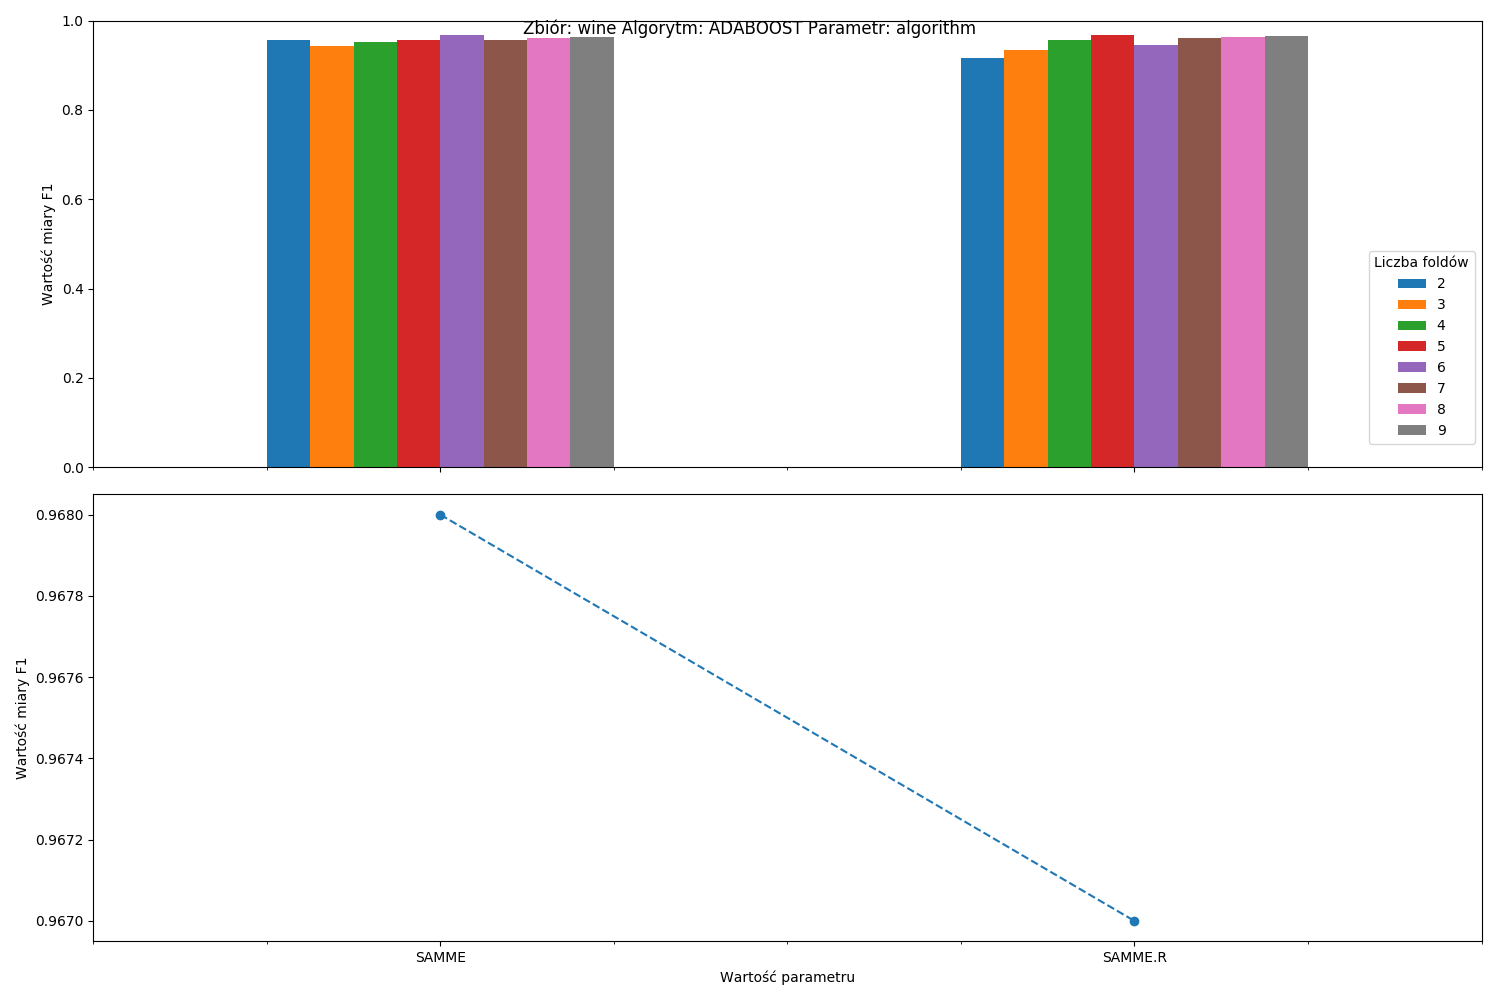
\includegraphics[width=\textwidth]{resources/plots/wine_adaboost_algorithm.png}
    \caption{Wykres wartości miary F1 dla zbioru "Wine" algorytmu "Adaboost" przy ustalonym parametrze "algorithm".}   
\end{figure}                    

\pagebreak

\begin{tabular}{llrrrrrrrr}
\hline
              & \{\} & \multicolumn{8}{l}{Miara F1} \\
              & Liczba foldów &        2 &      3 &      4 &      5 &      6 &      7 &      8 &      9 \\
Parametr & Wartość parametru &          &        &        &        &        &        &        &        \\
\hline
learning\_rate & 0.0001 &    0.934 &  0.918 &  0.972 &  0.972 &  0.973 &  0.928 &  0.962 &  0.966 \\
              & 0.001 &    0.955 &  0.945 &  0.962 &  0.972 &  0.973 &  0.956 &  0.972 &  0.945 \\
              & 0.01 &    0.933 &  0.946 &  0.945 &  0.955 &  0.900 &  0.946 &  0.977 &  0.956 \\
              & 0.1 &    0.950 &  0.924 &  0.934 &  0.950 &  0.939 &  0.984 &  0.978 &  0.968 \\
\hline
\end{tabular}

\begin{figure}[H]
    \center
    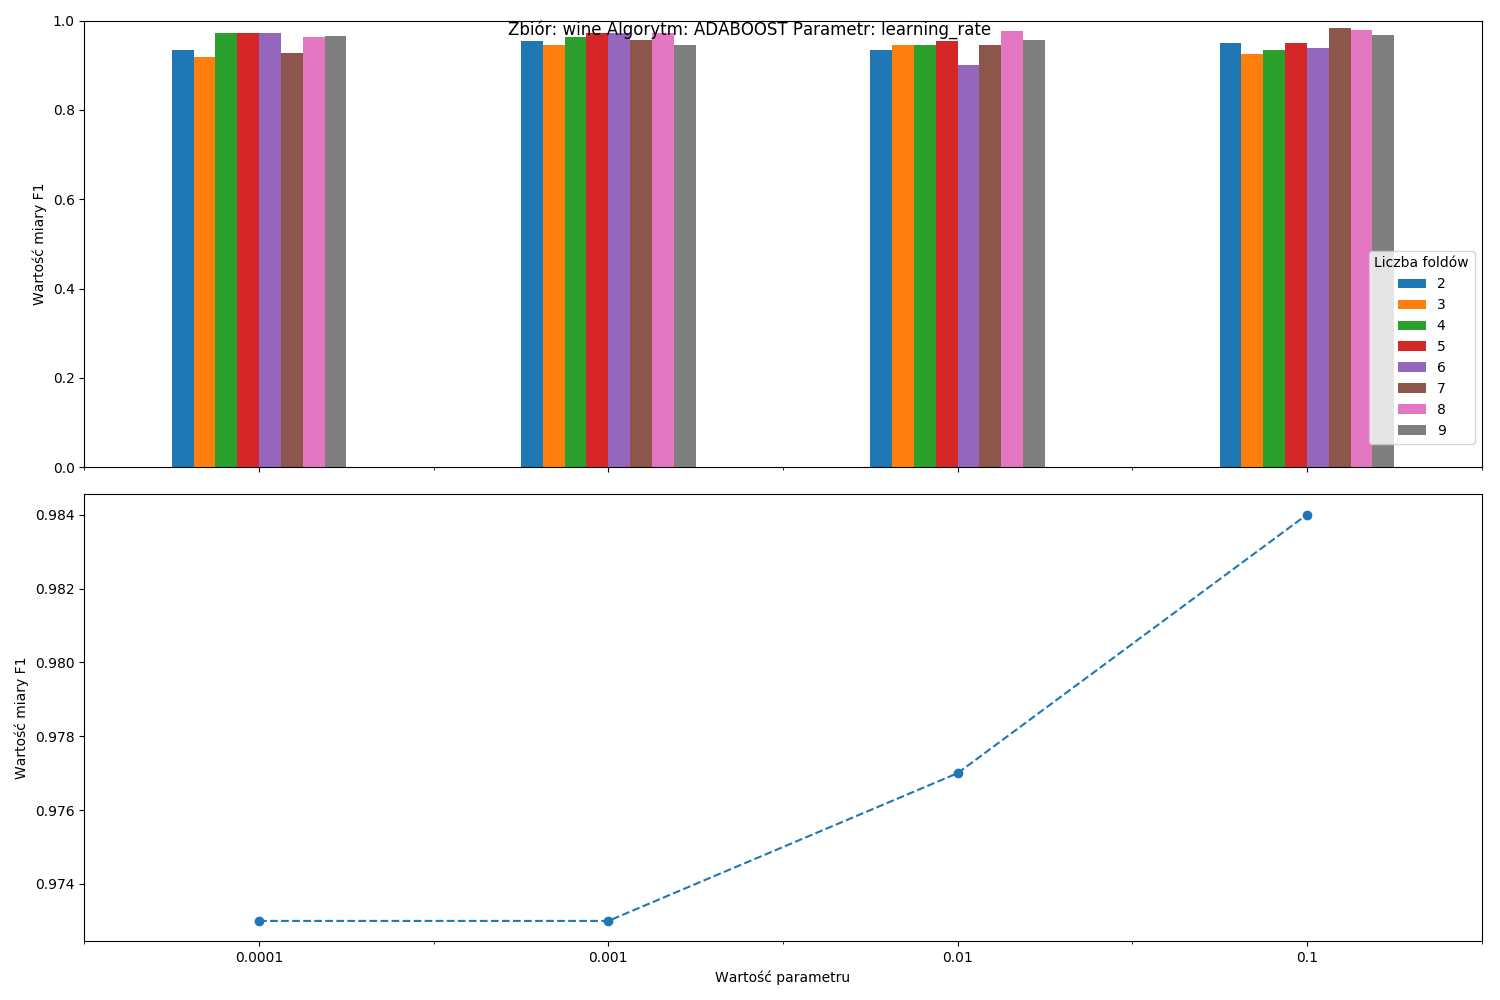
\includegraphics[width=\textwidth]{resources/plots/wine_adaboost_learning_rate.png}
    \caption{Wykres wartości miary F1 dla zbioru "Wine" algorytmu "Adaboost" przy ustalonym parametrze "learning\_rate".}
\end{figure}

\pagebreak
                    
\begin{tabular}{llrrrrrrrr}
\hline
             & \{\} & \multicolumn{8}{l}{Miara F1} \\
             & Liczba foldów &        2 &      3 &      4 &      5 &      6 &      7 &      8 &      9 \\
Parametr & Wartość parametru &          &        &        &        &        &        &        &        \\
\hline
n\_estimators & 10 &    0.928 &  0.896 &  0.968 &  0.966 &  0.973 &  0.967 &  0.966 &  0.962 \\
             & 25 &    0.972 &  0.939 &  0.944 &  0.955 &  0.949 &  0.962 &  0.977 &  0.962 \\
             & 50 &    0.928 &  0.927 &  0.957 &  0.967 &  0.939 &  0.972 &  0.960 &  0.955 \\
             & 75 &    0.945 &  0.945 &  0.946 &  0.977 &  0.968 &  0.979 &  0.938 &  0.966 \\
             & 99 &    0.950 &  0.917 &  0.979 &  0.961 &  0.961 &  0.961 &  0.968 &  0.960 \\
\hline
\end{tabular}

\begin{figure}[H]
    \center
    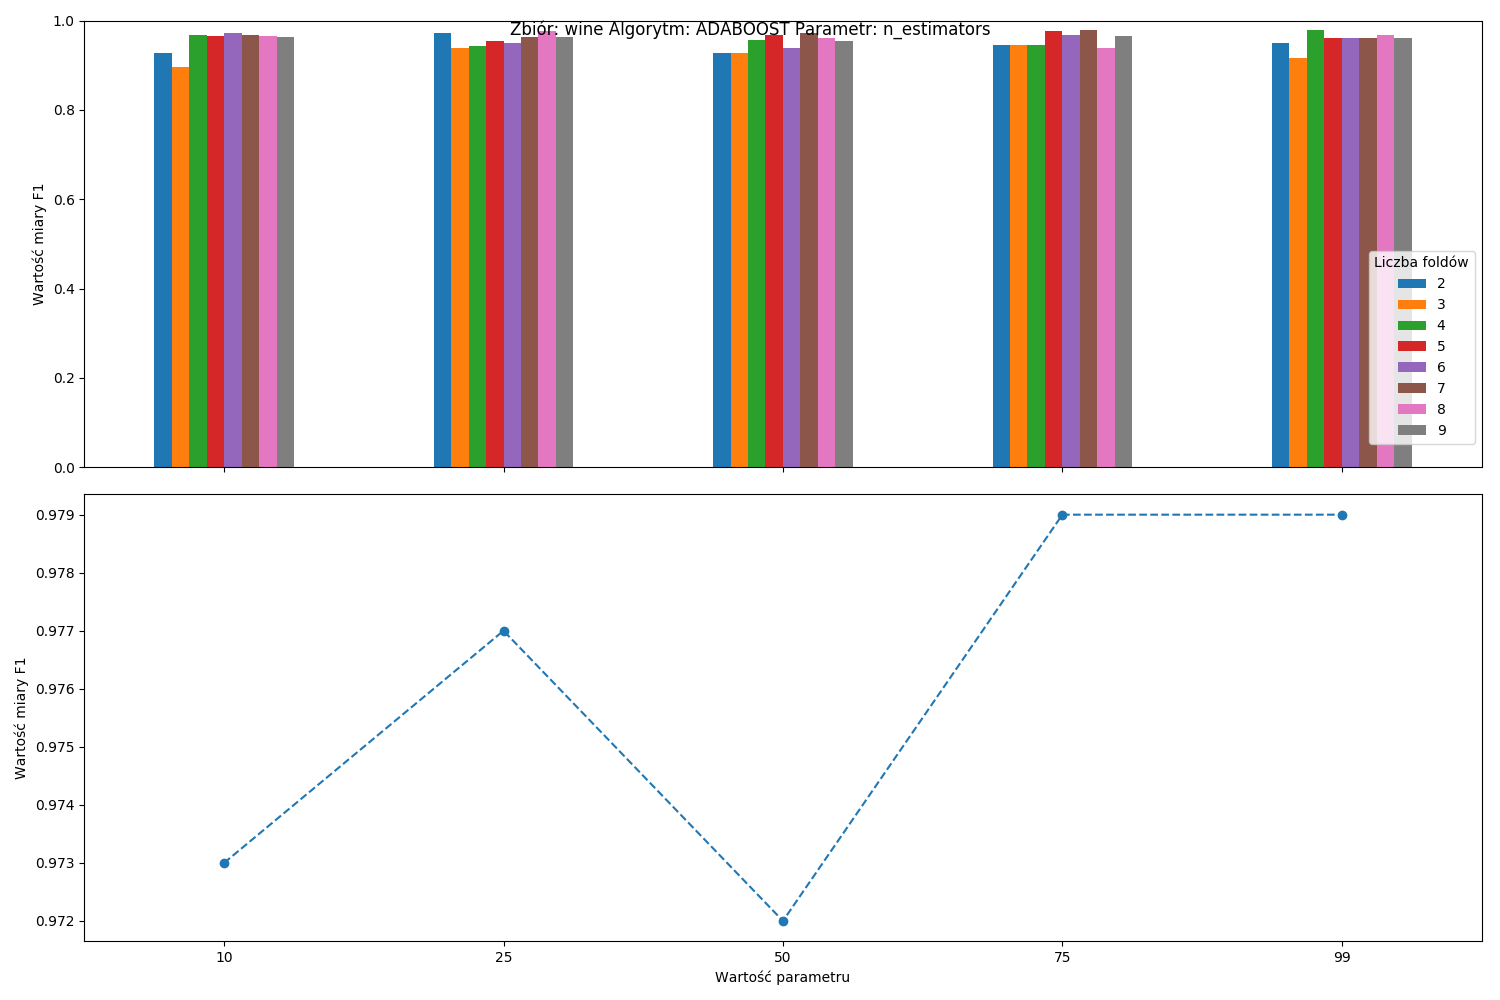
\includegraphics[width=\textwidth]{resources/plots/wine_adaboost_n_estimators.png}
    \caption{Wykres wartości miary F1 dla zbioru "Wine" algorytmu "Adaboost" przy ustalonym parametrze "n\_estimators".}
\end{figure}

\pagebreak
                    
\subsection{Algorytm Bagging}

\begin{tabular}{llrrrrrrrr}
\hline
          & \{\} & \multicolumn{8}{l}{Miara F1} \\
          & Liczba foldów &        2 &      3 &      4 &      5 &      6 &      7 &      8 &      9 \\
Parametr & Wartość parametru &          &        &        &        &        &        &        &        \\
\hline
bootstrap & False &    0.967 &  0.968 &  0.972 &  0.950 &  0.967 &  0.962 &  0.949 &  0.944 \\
          & True &    0.915 &  0.951 &  0.977 &  0.945 &  0.961 &  0.967 &  0.961 &  0.967 \\
\hline
\end{tabular}

\begin{figure}[H]
    \center
    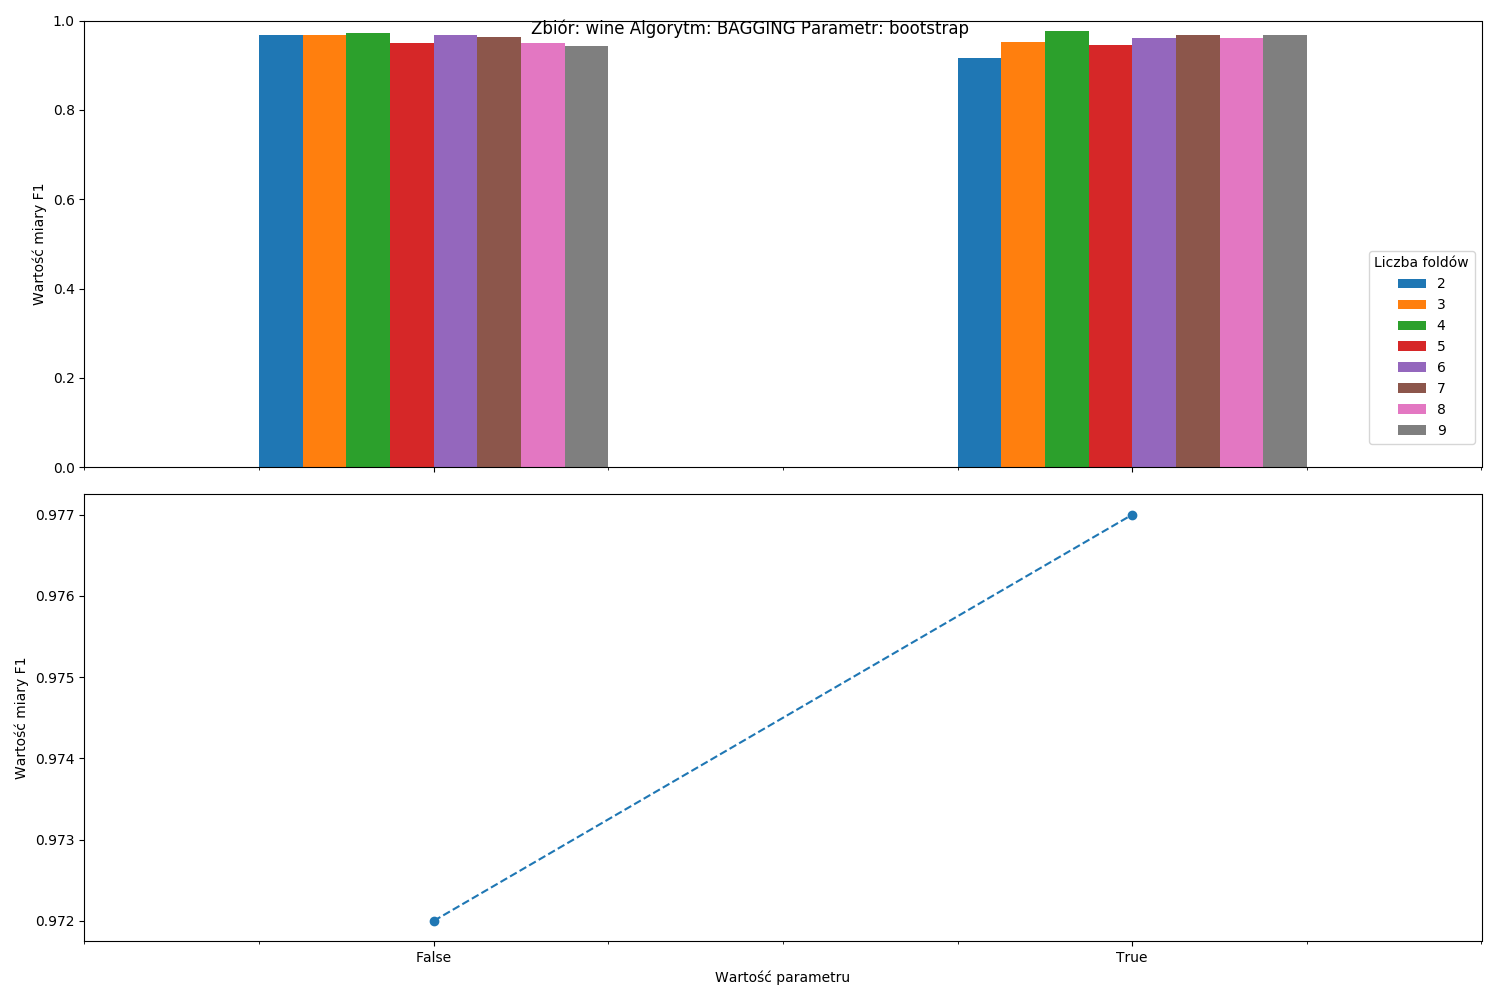
\includegraphics[width=\textwidth]{resources/plots/wine_bagging_bootstrap.png}
    \caption{Wykres wartości miary F1 dla zbioru "Wine" algorytmu "Bagging" przy ustalonym parametrze "bootstrap".}   
\end{figure}

\pagebreak
                    
\begin{tabular}{llrrrrrrrr}
\hline
            & \{\} & \multicolumn{8}{l}{Miara F1} \\
            & Liczba foldów &        2 &      3 &      4 &      5 &      6 &      7 &      8 &      9 \\
Parametr & Wartość parametru &          &        &        &        &        &        &        &        \\
\hline
max\_samples & 0.25 &    0.943 &  0.935 &  0.950 &  0.977 &  0.962 &  0.955 &  0.944 &  0.957 \\
            & 0.5 &    0.955 &  0.905 &  0.961 &  0.959 &  0.962 &  0.957 &  0.944 &  0.957 \\
            & 0.75 &    0.954 &  0.949 &  0.952 &  0.972 &  0.950 &  0.973 &  0.956 &  0.966 \\
            & 1.0 &    0.949 &  0.961 &  0.951 &  0.983 &  0.962 &  0.967 &  0.961 &  0.967 \\
\hline
\end{tabular}

\begin{figure}[H]
    \center
    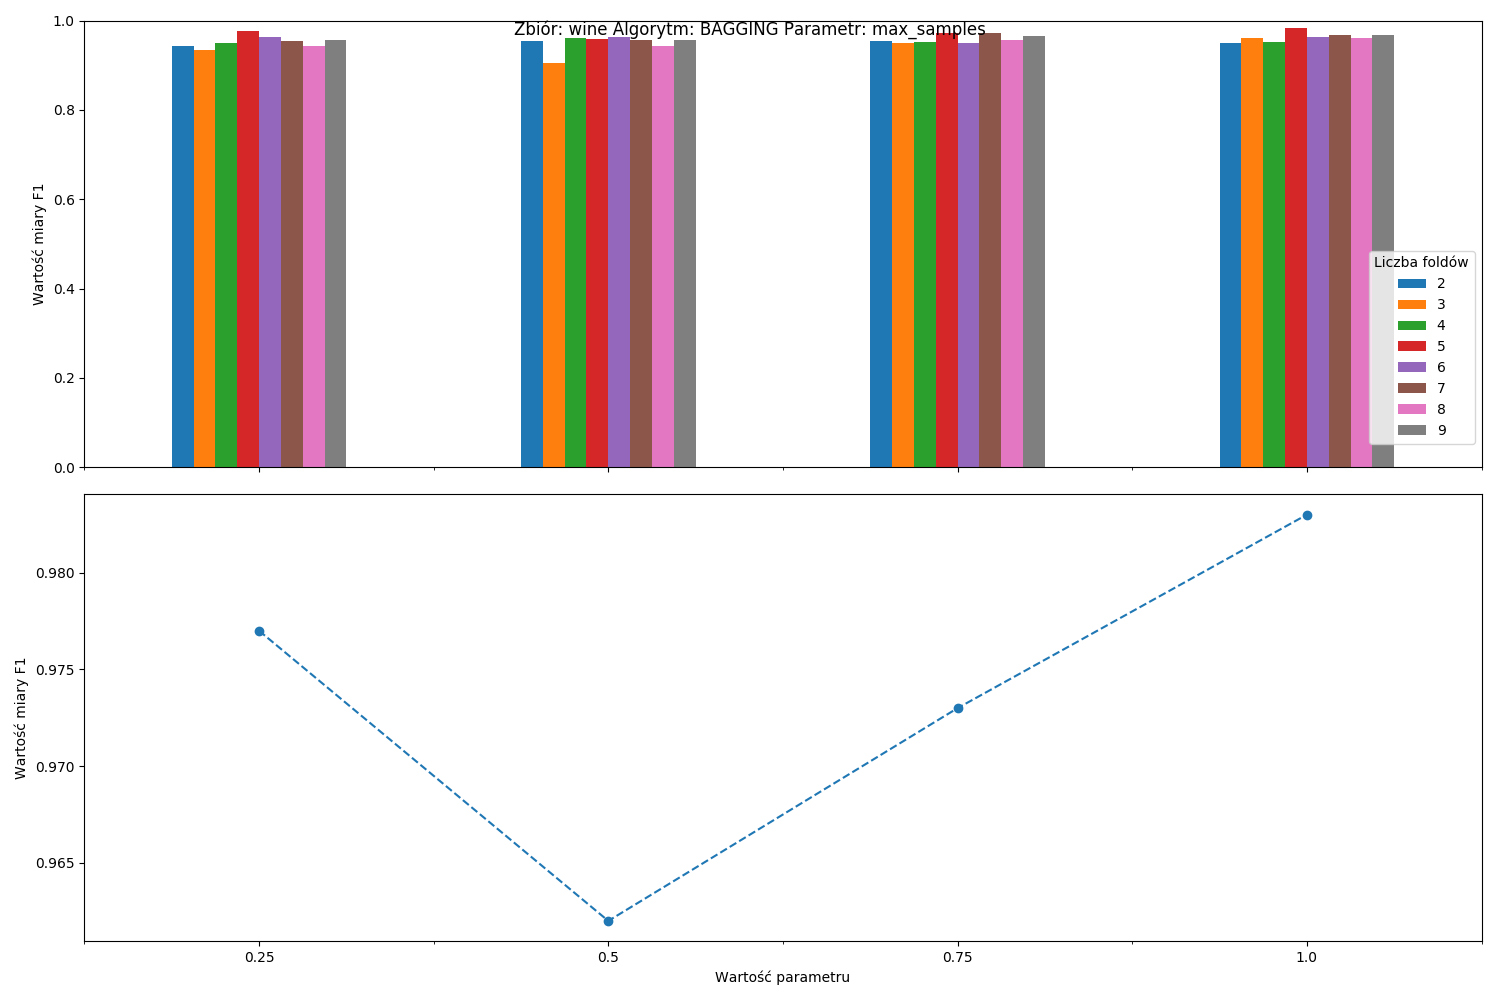
\includegraphics[width=\textwidth]{resources/plots/wine_bagging_max_samples.png}
    \caption{Wykres wartości miary F1 dla zbioru "Wine" algorytmu "Bagging" przy ustalonym parametrze "max\_samples".}
\end{figure}

\pagebreak
                    
\begin{tabular}{llrrrrrrrr}
\hline
             & \{\} & \multicolumn{8}{l}{Miara F1} \\
             & Liczba foldów &        2 &      3 &      4 &      5 &      6 &      7 &      8 &      9 \\
Parametr & Wartość parametru &          &        &        &        &        &        &        &        \\
\hline
n\_estimators & 10 &    0.955 &  0.940 &  0.967 &  0.966 &  0.967 &  0.961 &  0.961 &  0.973 \\
             & 25 &    0.915 &  0.979 &  0.968 &  0.966 &  0.962 &  0.967 &  0.951 &  0.962 \\
             & 50 &    0.934 &  0.915 &  0.962 &  0.966 &  0.961 &  0.968 &  0.949 &  0.950 \\
             & 75 &    0.983 &  0.966 &  0.937 &  0.968 &  0.955 &  0.966 &  0.971 &  0.972 \\
             & 99 &    0.949 &  0.939 &  0.935 &  0.944 &  0.967 &  0.957 &  0.966 &  0.950 \\
\hline
\end{tabular}

\begin{figure}[H]
    \center
    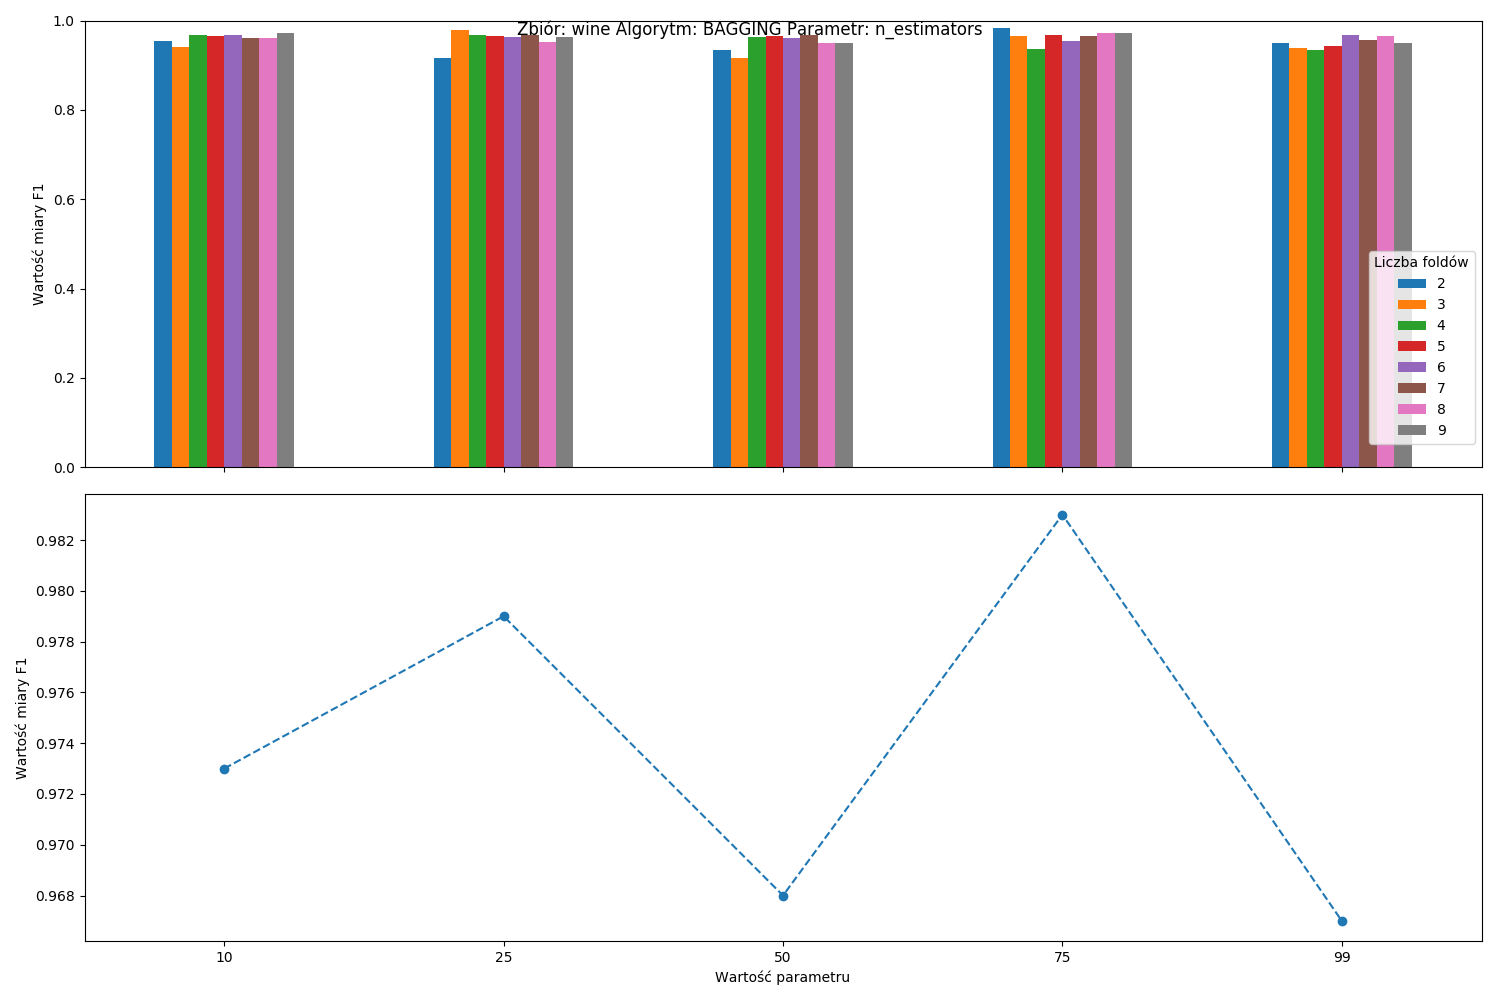
\includegraphics[width=\textwidth]{resources/plots/wine_bagging_n_estimators.png}
    \caption{Wykres wartości miary F1 dla zbioru "Wine" algorytmu "Bagging" przy ustalonym parametrze "n\_estimators".}
\end{figure}

\pagebreak
                    
\subsection{Algorytm Random-forest}

\begin{tabular}{llrrrrrrrr}
\hline
          & \{\} & \multicolumn{8}{l}{Miara F1} \\
          & Liczba foldów &        2 &      3 &      4 &      5 &      6 &      7 &      8 &      9 \\
Parametr & Wartość parametru &          &        &        &        &        &        &        &        \\
\hline
bootstrap & False &    0.978 &  0.941 &  0.972 &  0.967 &  0.961 &  0.974 &  0.978 &  0.957 \\
          & True &    0.973 &  0.945 &  0.955 &  0.956 &  0.949 &  0.979 &  0.938 &  0.950 \\
\hline
\end{tabular}

\begin{figure}[H]
    \center
    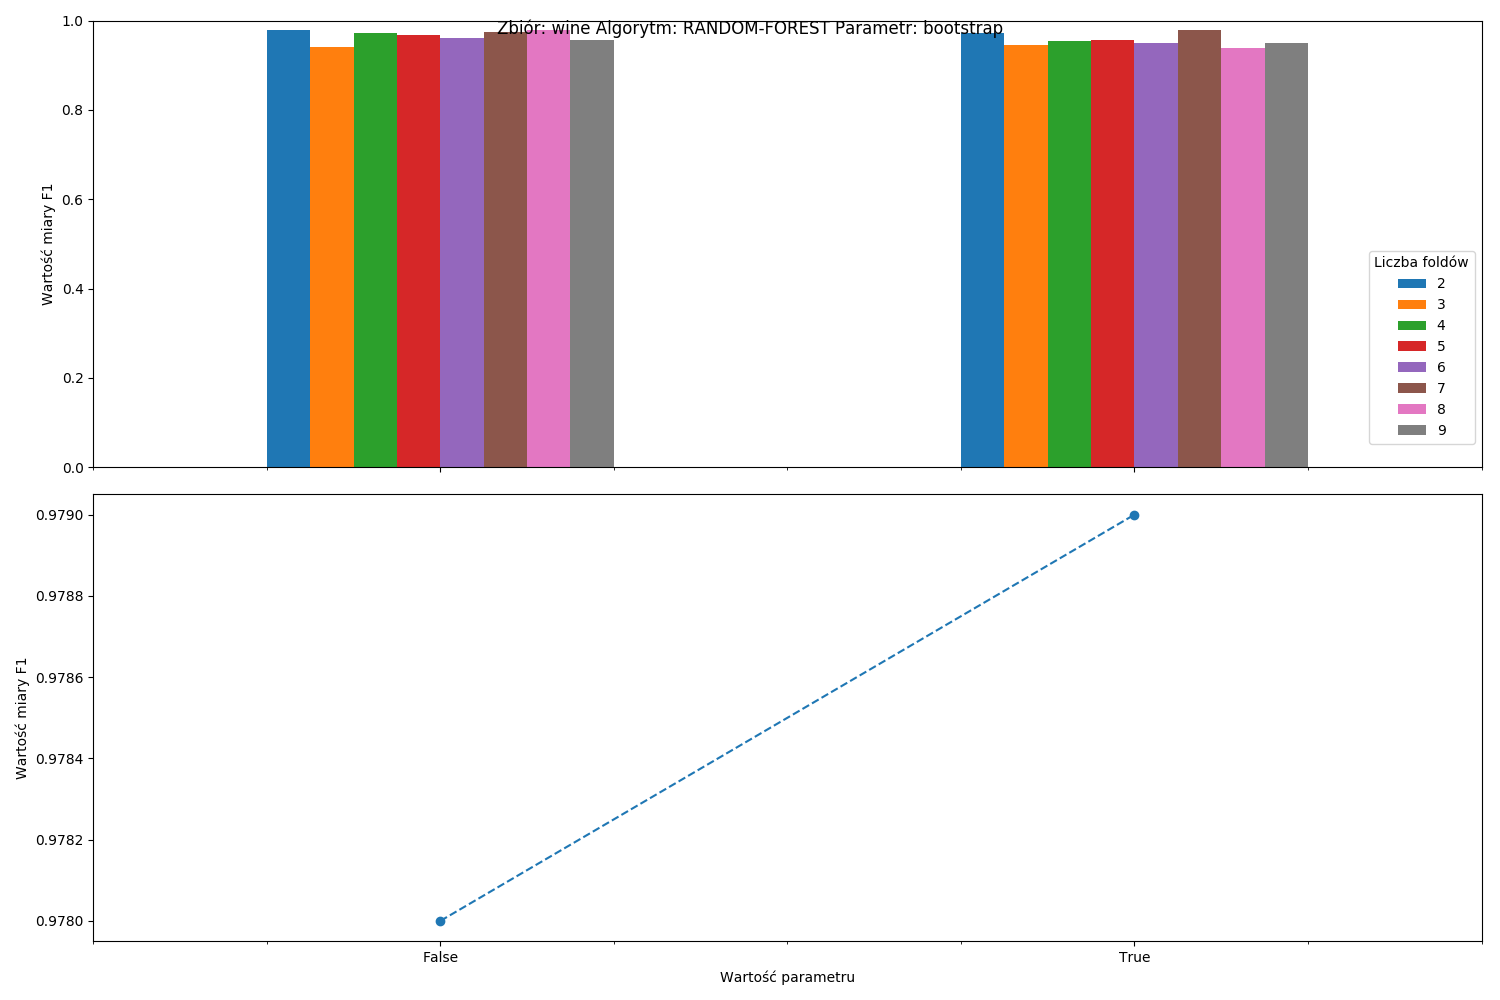
\includegraphics[width=\textwidth]{resources/plots/wine_random-forest_bootstrap.png}
    \caption{Wykres wartości miary F1 dla zbioru "Wine" algorytmu "Random-forest" przy ustalonym parametrze "bootstrap".}   
\end{figure}

\pagebreak
                    
\begin{tabular}{llrrrrrrrr}
\hline
          & \{\} & \multicolumn{8}{l}{Miara F1} \\
          & Liczba foldów &        2 &      3 &      4 &      5 &      6 &      7 &      8 &      9 \\
Parametr & Wartość parametru &          &        &        &        &        &        &        &        \\
\hline
criterion & entropy &    0.933 &  0.941 &  0.949 &  0.956 &  0.979 &  0.968 &  0.961 &  0.973 \\
          & gini &    0.950 &  0.954 &  0.951 &  0.955 &  0.973 &  0.967 &  0.961 &  0.962 \\
\hline
\end{tabular}

\begin{figure}[H]
    \center
    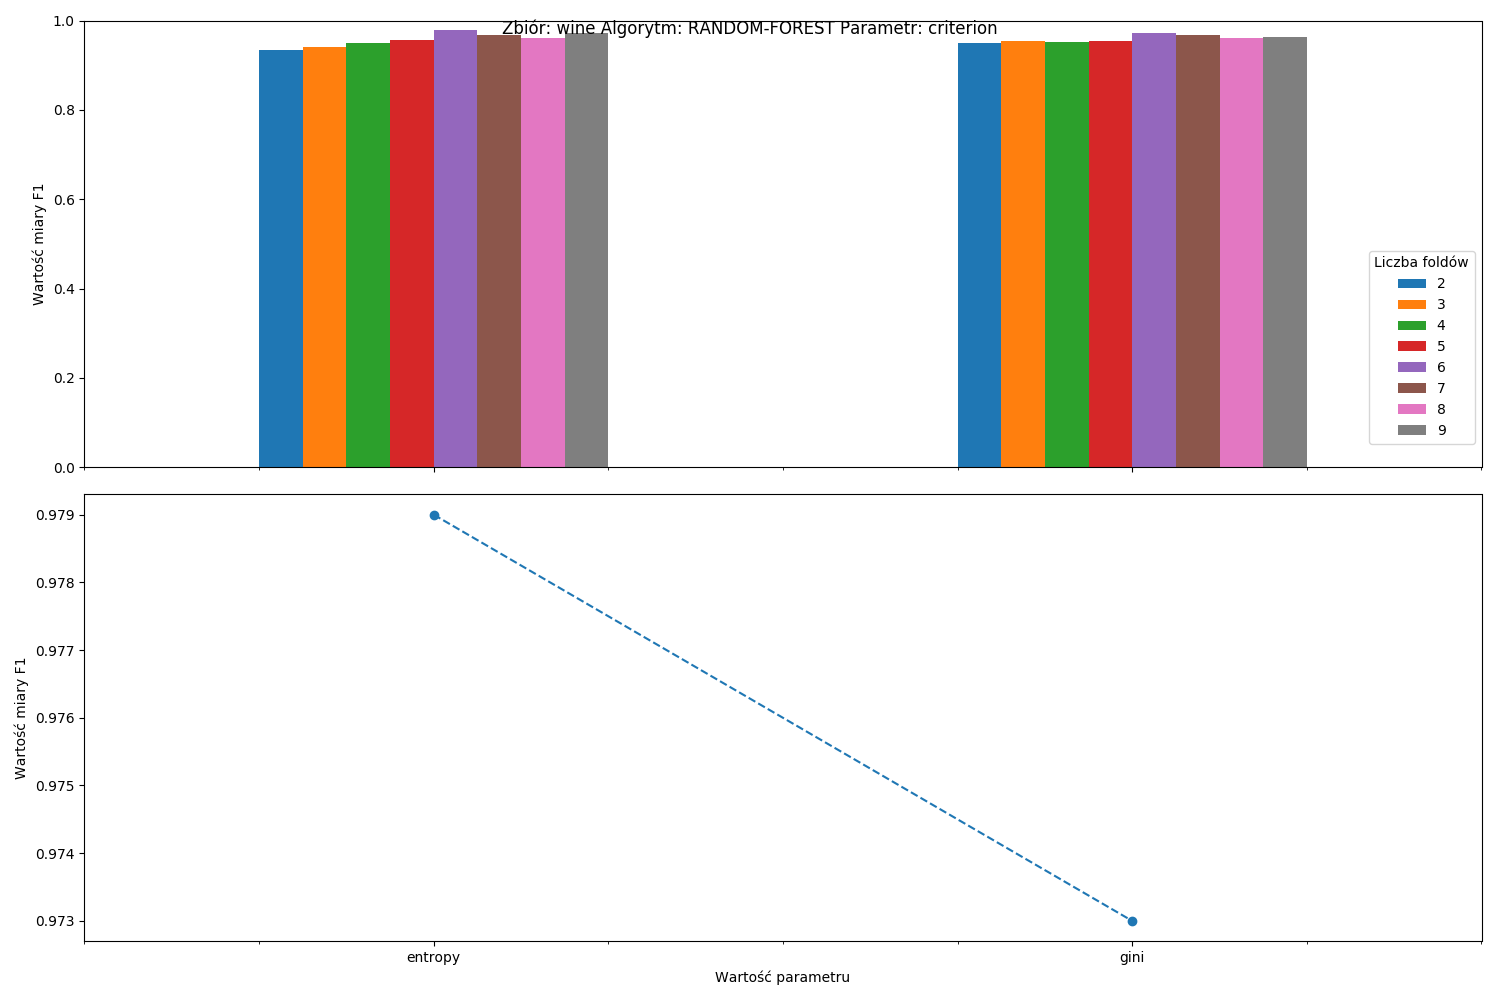
\includegraphics[width=\textwidth]{resources/plots/wine_random-forest_criterion.png}
    \caption{Wykres wartości miary F1 dla zbioru "Wine" algorytmu "Random-forest" przy ustalonym parametrze "criterion".}   
\end{figure}

\pagebreak
                    
\begin{tabular}{llrrrrrrrr}
\hline
             & \{\} & \multicolumn{8}{l}{Miara F1} \\
             & Liczba foldów &        2 &      3 &      4 &      5 &      6 &      7 &      8 &      9 \\
Parametr & Wartość parametru &          &        &        &        &        &        &        &        \\
\hline
n\_estimators & 10 &    0.951 &  0.913 &  0.939 &  0.961 &  0.968 &  0.984 &  0.972 &  0.979 \\
             & 25 &    0.945 &  0.929 &  0.960 &  0.950 &  0.968 &  0.956 &  0.951 &  0.961 \\
             & 50 &    0.951 &  0.907 &  0.963 &  0.972 &  0.979 &  0.984 &  0.972 &  0.966 \\
             & 75 &    0.961 &  0.919 &  0.947 &  0.961 &  0.967 &  0.950 &  0.943 &  0.966 \\
             & 99 &    0.950 &  0.961 &  0.972 &  0.978 &  0.955 &  0.956 &  0.941 &  0.973 \\
\hline
\end{tabular}

\begin{figure}[H]
    \center
    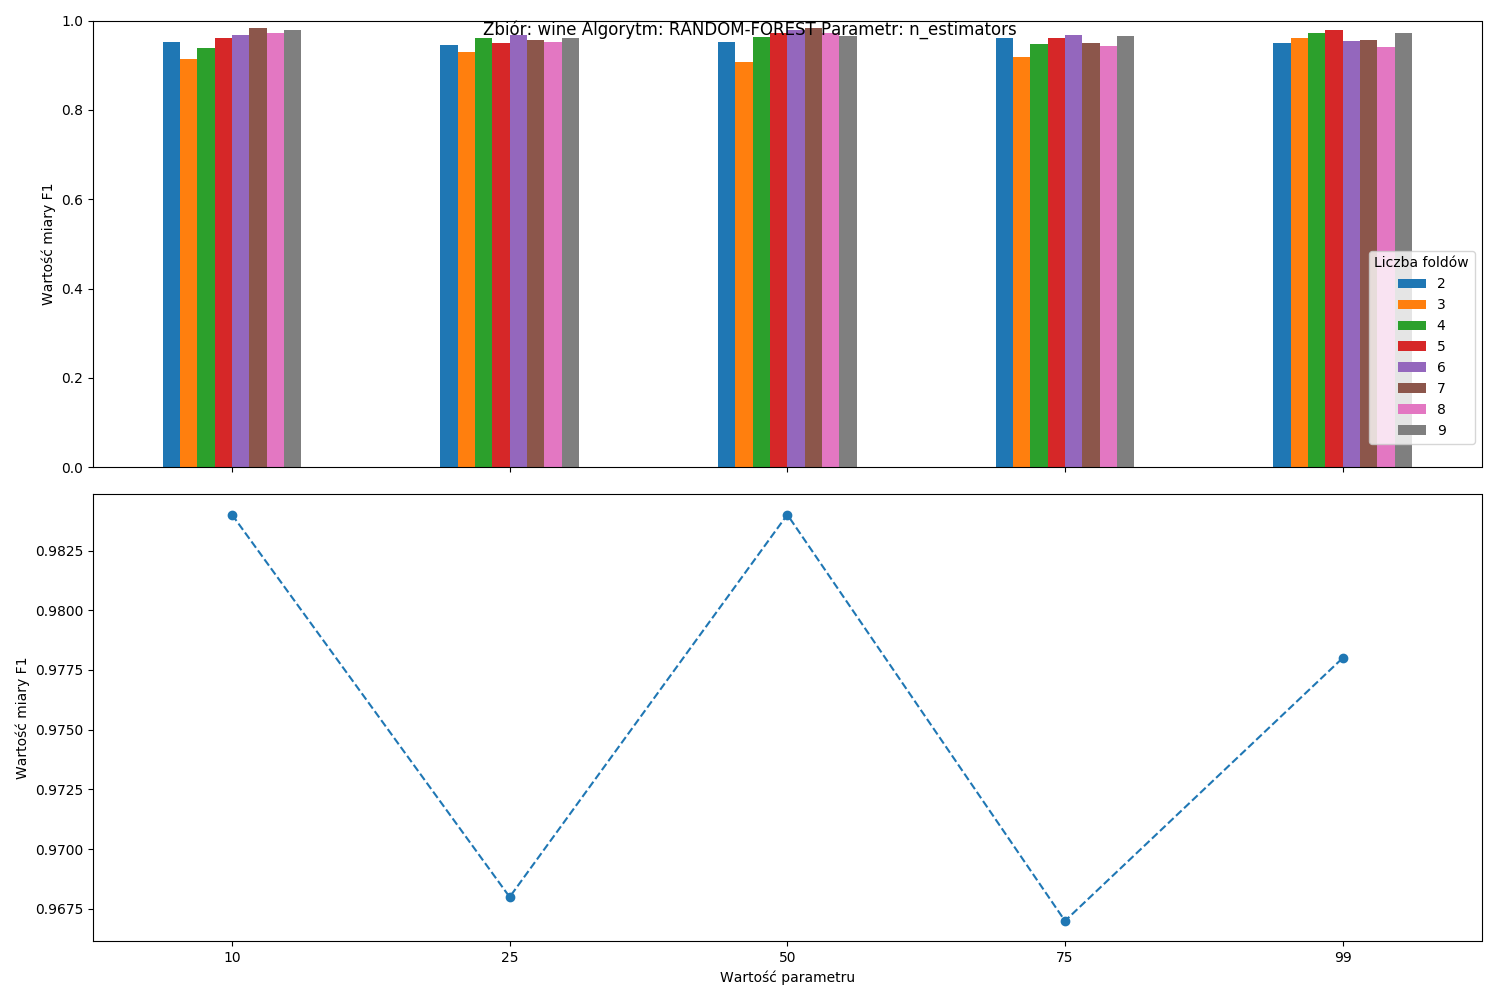
\includegraphics[width=\textwidth]{resources/plots/wine_random-forest_n_estimators.png}
    \caption{Wykres wartości miary F1 dla zbioru "Wine" algorytmu "Random-forest" przy ustalonym parametrze "n\_estimators".}
\end{figure}                    
                    
\pagebreak

\begin{tabular}{llrrrrrrrr}
\hline
             & \{\} & \multicolumn{8}{l}{Miara F1} \\
             & Liczba foldów &        2 &      3 &      4 &      5 &      6 &      7 &      8 &      9 \\
Parametr & Wartość parametru &          &        &        &        &        &        &        &        \\
\hline
max\_features & 0.25 &    0.922 &  0.937 &  0.911 &  0.925 &  0.928 &  0.950 &  0.933 &  0.940 \\
             & 0.5 &    0.920 &  0.908 &  0.956 &  0.944 &  0.946 &  0.941 &  0.973 &  0.962 \\
             & 0.75 &    0.944 &  0.868 &  0.950 &  0.944 &  0.943 &  0.952 &  0.968 &  0.957 \\
             & 1.0 &    0.893 &  0.934 &  0.940 &  0.939 &  0.949 &  0.921 &  0.938 &  0.957 \\
\hline
\end{tabular}

\begin{figure}[H]
    \center
    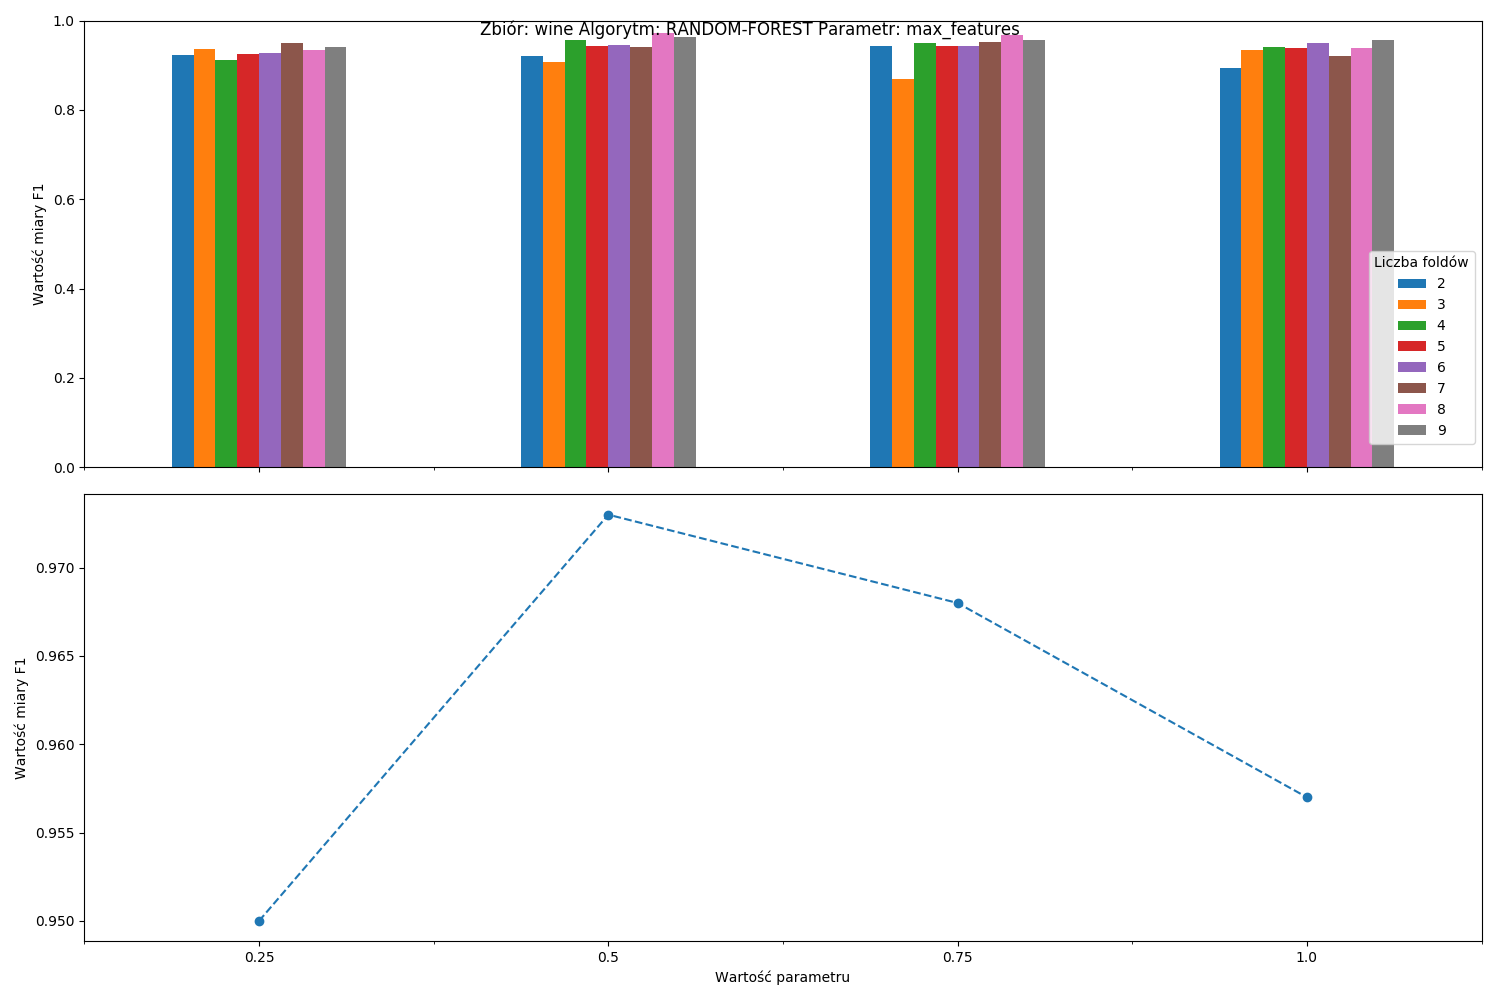
\includegraphics[width=\textwidth]{resources/plots/wine_random-forest_max_features.png}
    \caption{Wykres wartości miary F1 dla zbioru "Wine" algorytmu "Random-forest" przy ustalonym parametrze "max\_features".}
\end{figure}

\pagebreak